\documentclass{standalone}

\usepackage{tikz}
\usetikzlibrary{
  shapes,
  arrows,
  shapes.geometric,
  positioning,
}

% Define block styles
\tikzstyle{parameter} = [
rectangle,
draw,
fill=red!20,
text width=2.75cm,
text badly centered,
rounded corners
]

\tikzstyle{calculated} = [
rectangle,
draw,
text width=2.75cm,
text badly centered,
rounded corners
]

\tikzstyle{result} = [
rectangle,
draw,
fill=blue!20,
text width=2.75cm,
text badly centered,
rounded corners
]

\tikzstyle{arrow} = [draw, -latex']
\tikzstyle{noarrow} = [draw, dashed]

% set consistent font size
\tikzset{every picture/.style={font issue=\footnotesize},
         font issue/.style={execute at begin picture={#1\selectfont}}
         }

\begin{document}

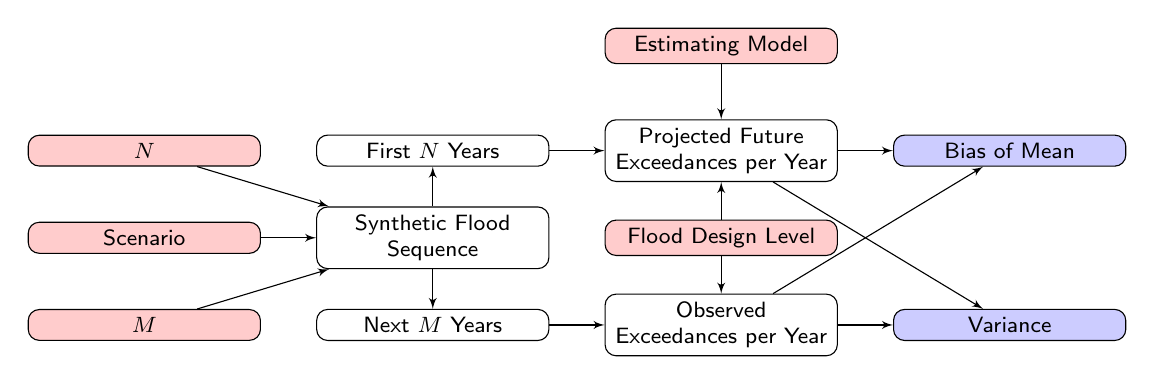
\begin{tikzpicture}[node distance = 0.7cm, auto, font=\sffamily]
  % Place nodes
  \node [parameter] (genmod) {Scenario};
  \node [parameter, above=of genmod] (N) {$N$};
  \node [parameter, below=of genmod] (M) {$M$};
  
  \node [calculated, right=of genmod] (seq) {Synthetic Flood Sequence};
  \node [calculated, right=of N] (historical) {First $N$ Years};
  \node [calculated, right=of M] (future) {Next $M$ Years};

  \node [calculated, right=of historical] (pThat) {Projected Future Exceedances per Year};
  \node [calculated, right= of future] (pT) {Observed Exceedances per Year};

  \node [parameter, above=of pThat] (fitting) {Estimating Model};
  \node [parameter, right=of seq] (threshold) {Flood Design Level};

  \node [result, right=of pThat] (bias) {Bias of Mean};
  \node [result, right=of pT] (variance) {Variance};
  
  % Draw edges
  \path [arrow] (N) -- (seq);
  \path [arrow] (M) -- (seq);
  \path [arrow] (genmod) -- (seq);

  \path [arrow] (seq) -- (historical);
  \path [arrow] (seq) -- (future);

  \path [arrow] (future) -- (pT);
  \path [arrow] (historical) -- (pThat);
  \path [arrow] (fitting) -- (pThat);

  \path [arrow] (threshold) -- (pThat);
  \path [arrow] (threshold) -- (pT);

  \path[arrow] (pThat) -- (bias);
  \path[arrow] (pT) -- (bias);
  \path[arrow] (pThat) -- (variance);
  \path[arrow] (pT) -- (variance);
 
\end{tikzpicture}


\end{document}
%%% Local Variables:
%%% mode: latex
%%% TeX-master: t
%%% End:
